

In this section, we evaluate the type-I error and the statistical power of signature-based test statistics, using synthetic anomalous diffusion data and real-world molecular biology data.

\subsection{Anomalous diffusions}\label{sec:anomalousDiffs}

We consider the problem of distinguishing Brownian motion (BM) from BM perturbed by an impulsive spike occurring at a uniformly random time. This example, connected to the theory of Brownian fast points \citep{davis1985brownian}, has been introduced by \citet{davis1984randomly} and \citet{hitchcock1992some}, and has also been empirically examined by \citet{cass2024variance}. For a given sample path $X$, we consider the hypothesis test
\begin{equation*}
H_0: X\sim\mu  \text{ against } 
        H_1: X\sim\nu_\varepsilon,
\end{equation*}
 with~$\mu$ the law of Brownian motion on $[0,2]$ and $\nu_\varepsilon$ that of a process with a spike. Following the presentation in \cite[Chapter 6]{hitchcock1992some},
 define the alternative process
$$
X^\varepsilon_t=B_t+\varepsilon\sqrt{[t-\theta]^+}\wedge 1, \quad\text{for } t\in [0,2],
$$
where $\theta$ is a random time drawn from the uniform distribution on $[0,1]$, $\varepsilon>0$ controls the magnitude of the spike, and $[x]^+=\max\{x,0\}$. Our numerical studies show how our detection procedure—based on signature transforms of the paths—can distinguish between~$\mu$ and~$\nu_\varepsilon$ for different intensities~$\varepsilon$ using the Area Under the Receiver Operating Characteristic curve (AUROC) as performance metric. We expect that as $\varepsilon$ increases, the spike gets more pronounced and produces a clearer non-Brownian signature, leading to higher detection power. When $\varepsilon \approx 0$, the spike is subtle so detection is more challenging.

\citet{hitchcock1992some} established that there is a critical value for the intensity parameter $\varepsilon$. When $\varepsilon < \sqrt{8}$, the measure corresponding to the process with a spike remains absolutely continuous with respect to the measure of standard Brownian motion. Conversely, when $\varepsilon > \sqrt{8}$ the two measures become singular. In our experiments, using the distance to the expected signature as test statistic, we do not observe an abrupt phase transition precisely at $\varepsilon=\sqrt{8}$. Instead, the AUROC improves gradually as~$\varepsilon$ increases 
(Figure~\ref{fig:auroc}). 

\begin{figure}[h]
    \centering
\begin{subfigure}{0.45\textwidth}
    \centering 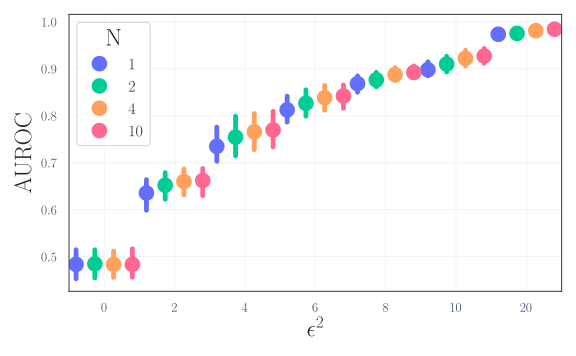
\includegraphics[width=1.\linewidth]{figures/Depth_spike_AUROC.png}
\caption{}\label{fig:auroc}
\end{subfigure}
\begin{subfigure}{0.45\textwidth}
    \centering
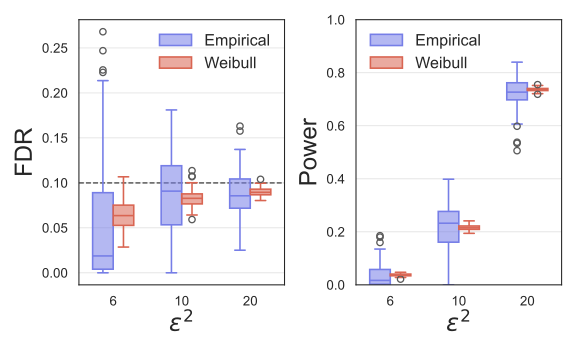
\includegraphics[width=1.\linewidth]{figures/fdr_power_depth_trunc5.png}
\caption{}\label{fig:fdr}
\end{subfigure}
\begin{subfigure}{0.45\textwidth}
    \centering
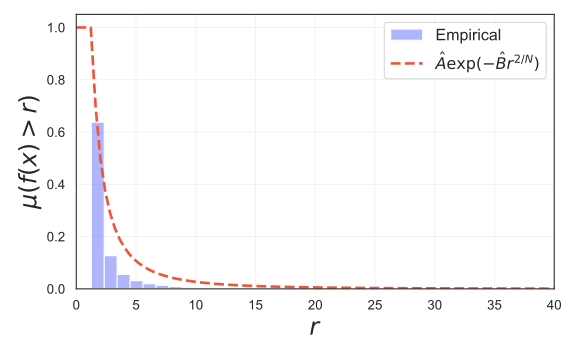
\includegraphics[width=1.\linewidth]{figures/Weibull_fit.png}
\caption{}\label{fig:weibull_fit}
\end{subfigure}
\begin{subfigure}{0.45\textwidth}
    \centering
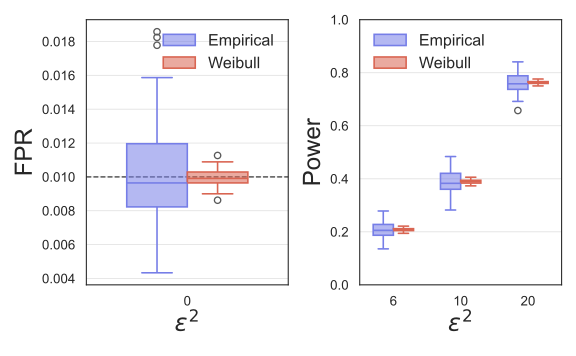
\includegraphics[width=1.\linewidth]{figures/fpr_power_depth_trunc5.png}
\caption{}\label{fig:fpr}
\end{subfigure}
    \caption{\textbf{Brownian motion perturbed by a  spike.} (a) AUROC as a function of the spike intensity for the distance to the expected signature. (b) Multiple testing false discovery rate and power at level $\alpha=0.1$ comparing empirical p-values (from 1,000 samples) with p-values obtained from a Weibull tail-bound fitted using 100,000 samples. (c) Weibull tail-bound fit (d) Single hypothesis false positive rate and power at level $\alpha=0.01$. }
    \label{fig:placeholder}
\end{figure}

Next, to evaluate the type-I error rate and the power, we simulate $J=100$ researchers. Each researcher $j$ has an independent fixed dataset $D_j$ of $n=2000$ Brownian motion sample paths and $L=50$ test sets $D^\text{test}_{j,l}$ 
(for $l=1,\ldots, L$)
of $n_\text{test}=1000$ Brownian motion sample paths, with $10\%$ of outliers (Brownian motion perturbed by a spike). Each researcher divides its reference dataset $D_j$ into $1000$ sample paths to estimate the expected signature of Brownian motion and $1000$ sample paths to estimate the p-values of all observations across all test datasets $D_{j,l}$. To measure the false discovery rate (FDR), the Benjamini-Hochberg procedure~\citep{benjamini1995controlling} is applied to all p-values in $D_{j,l}$ at level $\alpha=0.10$, the false positive rate (FPR) is then estimated, and averaged over the $L$ test datasets. Similarly, a statistical estimate for the power is obtained. To estimate the false positive rate, the raw  p-values are thresholded at level $\alpha=0.01$. 

As can be seen on Figures~\ref{fig:fdr} and~\ref{fig:fpr}, which show the FDR and FPR for different values of the signal strength $\varepsilon^2$, both methods control the marginal FDR and FPR at the desired levels. We also compared to a parametric approach (Weibull), where we fit a curve $A\exp(-Br^{2/N})$ to the tail of the reference measure estimated with a relatively large number of samples, leveraging the results from \Cref{ssec:probabilistic_estimates}. As can be seen on  on Figure~\ref{fig:fdr}, this parametric approach controls the conditional FDR and FPR for a greater proportion of researchers. As expected, the false positive rate exhibits a lower variance (Figure~\ref{fig:fpr}) when the Weibull parametric approach is used.


\begin{figure}[h]
    \centering
    \begin{subfigure}{0.49\textwidth}
     \centering
         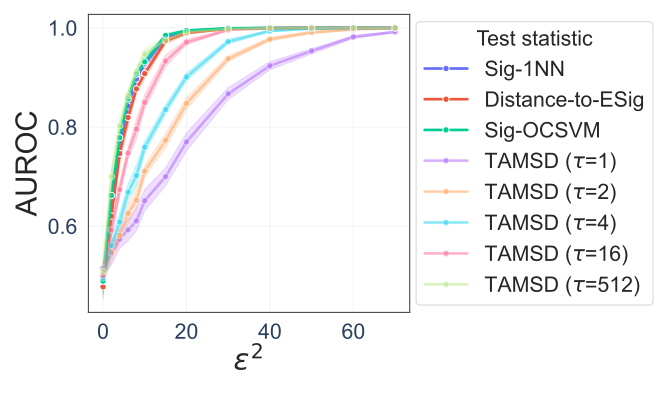
\includegraphics[width=1\linewidth]{figures/comparison_spike_AUROC_bigger.png}
    \caption{}
    \label{fig:placeholder}
    \end{subfigure}
       \begin{subfigure}{0.49\textwidth}
     \centering
         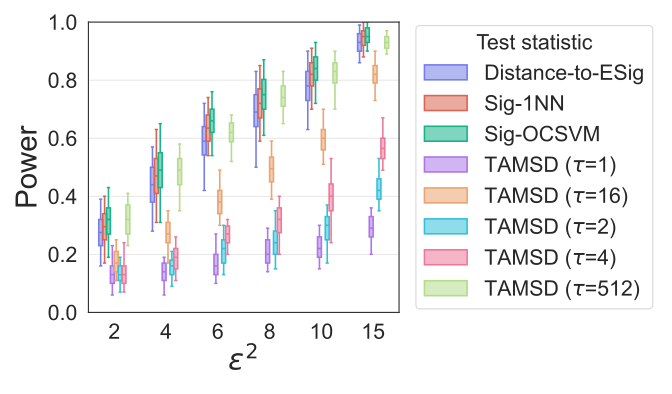
\includegraphics[width=1\linewidth]{figures/comparison_spike_power_at_0_1_bigger.png}
    \caption{}
    \label{fig:placeholder}
    \end{subfigure}
    \caption{\textbf{Comparison of different test statistics.} Comparison of \acrshort{ocsvm}, conformance score, distance to the expected signature, and TAMSD with $\tau\in\{1,2,4,16,512\}$.}
\end{figure}

Finally, we compare our signature-based test statistics with another test statistic for detecting anomalous diffusions from the literature \citep{sikora2017mean} given by the time-averaged mean square displacement (TAMSD)
\begin{align}
    M_N(\tau) := \frac{1}{N-\tau}\sum_{j=1}^{N-\tau}(X(j+\tau)-X(j))^2.
\end{align}
The TAMSD scales as $M_N(\tau)\sim \tau ^\alpha$ with $\alpha=2H$ for fractional Brownian motion with Hurst index $H \in (0,1)$.
Brownian motion has a linear power-law growth of the mean squared displacement in the course of time. 


\subsection{Anomaly detection in RNA direct sequencing data}

In molecular biology, a central challenge is to detect non-canonical nucleotides on RNA molecules, i.e. bases chemically modified relative to the four standard nucleotides (A, U, G, C). Mapping such modifications has become a major research focus, as they have been found to modulate crucial cellular processes and are increasingly linked to human diseases, ranging from neurodevelopmental disorders to cancer. 
Recently, significant progress has been achieved by leveraging Nanopore direct sequencing data \citep{white2022modification,furlan2021computational}. Nanopore sequencing transduces long RNA polymers into an electrical signal and chemical modifications have been shown to induce characteristic alterations in the measured signal. Most prior approaches have focused on training neural network based classifiers on known modification types. However, since many modifications remain unknown or poorly characterised, this is also naturally cast as a novelty detection task \cite{lemercier2025path}.


\begin{figure}[h]
    \centering
    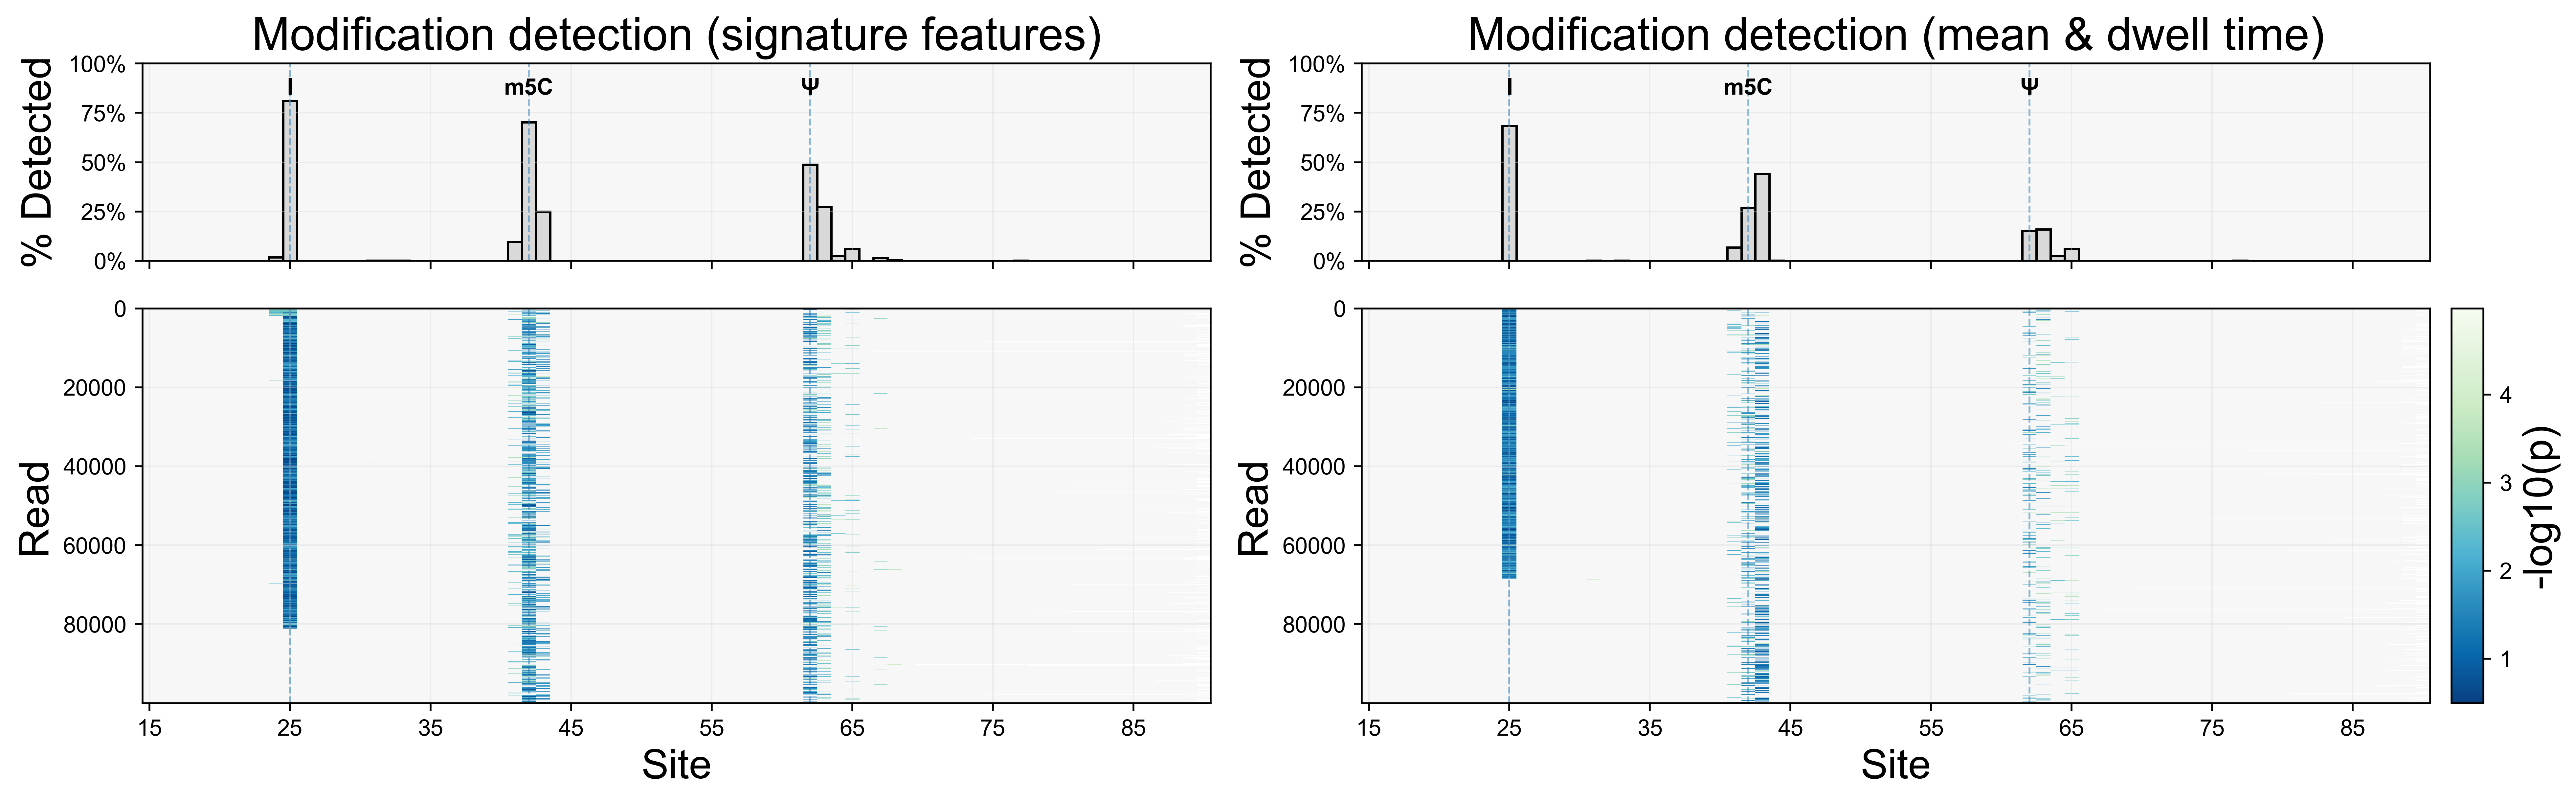
\includegraphics[width=1\linewidth]{figures/rna_results.png}
    \caption{\textbf{Modification detection in nanopore reads with \acrshort{ocsvm}.} Bottom: per-read p-values (with multiple testing correction) at each site; non-significant p-values at level 0.20 are rendered light grey. Top: for each site, the proportion of significant reads. \emph{Left:} signature features. \textit{Right:} mean-current and dwell-time features.}
    \label{fig:RNA}
\end{figure}


Here, we analyse short synthetic oligonucleotides, i.e., RNA molecules chemically synthesised in a laboratory. In this controlled setting, three distinct chemical modifications were introduced at defined positions within a 100-nucleotide sequence \citep{leger2021rna}
\begin{figure}[H]
    \centering
    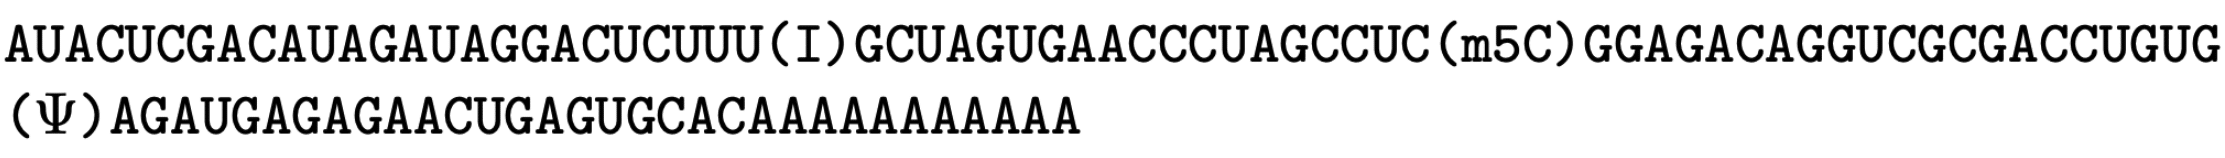
\includegraphics[width=1\linewidth]{figures/mintedBit.png}
\end{figure}
%\begin{minted}[escapeinside=||]{text}
%AUACUCGACAUAGAUAGGACUCUUU(I)GCUAGUGAACCCUAGCCUC(m5C)GGAGACAGGUCGCGACCUGUG
%(|$\Psi$|)AGAUGAGAGAACUGAGUGCACAAAAAAAAAAA
%\end{minted}
The raw nanopore direct sequencing data were obtained from the European Nucleotide Archive (accession number PRJEB44511). It contains an unmodified sample and a sample where the three modifications have been deposited. Basecalling and signal processing were performed using Dorado\footnote{\url{https://github.com/nanoporetech/dorado}}, read alignment was carried out with minimap2 \citep{li2018minimap2}, and event-level signal segmentation was obtained with Uncalled4 \citep{kovaka2025uncalled4}, yielding segmented time series representations for our analysis. 

We compared a \acrshort{ocsvm} using signatures truncated at level $N=6$ after applying two path transforms (the \emph{time augmentation} and the \emph{invisibility-reset} transforms \citep{lyons2025signature} and a \acrshort{ocsvm} trained on two standard nanopore features given by the signal duration (commonly referred to as the \emph{dwell time}) and signal mean value. We fitted the \acrshort{ocsvm} using $3\,000$ reads from the unmodified sample for each site, and computed the empirical p-values using $100\,000$ other unmodified reads. Figure~\ref{fig:RNA} shows that, at a Benjamini–Hochberg FDR level of 0.20 (with Storey correction), the signature-feature model yields consistently higher recall for all three modification types, namely inosine (I), 5-methylcytosine (m5C), and pseudouridine ($\Psi$).



